\documentclass[final,9pt,fleqn]{beamer}\usepackage[]{graphicx}\usepackage[]{xcolor}
% maxwidth is the original width if it is less than linewidth
% otherwise use linewidth (to make sure the graphics do not exceed the margin)
\makeatletter
\def\maxwidth{ %
  \ifdim\Gin@nat@width>\linewidth
    \linewidth
  \else
    \Gin@nat@width
  \fi
}
\makeatother

\definecolor{fgcolor}{rgb}{0.345, 0.345, 0.345}
\newcommand{\hlnum}[1]{\textcolor[rgb]{0.686,0.059,0.569}{#1}}%
\newcommand{\hlsng}[1]{\textcolor[rgb]{0.192,0.494,0.8}{#1}}%
\newcommand{\hlcom}[1]{\textcolor[rgb]{0.678,0.584,0.686}{\textit{#1}}}%
\newcommand{\hlopt}[1]{\textcolor[rgb]{0,0,0}{#1}}%
\newcommand{\hldef}[1]{\textcolor[rgb]{0.345,0.345,0.345}{#1}}%
\newcommand{\hlkwa}[1]{\textcolor[rgb]{0.161,0.373,0.58}{\textbf{#1}}}%
\newcommand{\hlkwb}[1]{\textcolor[rgb]{0.69,0.353,0.396}{#1}}%
\newcommand{\hlkwc}[1]{\textcolor[rgb]{0.333,0.667,0.333}{#1}}%
\newcommand{\hlkwd}[1]{\textcolor[rgb]{0.737,0.353,0.396}{\textbf{#1}}}%
\let\hlipl\hlkwb

\usepackage{framed}
\makeatletter
\newenvironment{kframe}{%
 \def\at@end@of@kframe{}%
 \ifinner\ifhmode%
  \def\at@end@of@kframe{\end{minipage}}%
  \begin{minipage}{\columnwidth}%
 \fi\fi%
 \def\FrameCommand##1{\hskip\@totalleftmargin \hskip-\fboxsep
 \colorbox{shadecolor}{##1}\hskip-\fboxsep
     % There is no \\@totalrightmargin, so:
     \hskip-\linewidth \hskip-\@totalleftmargin \hskip\columnwidth}%
 \MakeFramed {\advance\hsize-\width
   \@totalleftmargin\z@ \linewidth\hsize
   \@setminipage}}%
 {\par\unskip\endMakeFramed%
 \at@end@of@kframe}
\makeatother

\definecolor{shadecolor}{rgb}{.97, .97, .97}
\definecolor{messagecolor}{rgb}{0, 0, 0}
\definecolor{warningcolor}{rgb}{1, 0, 1}
\definecolor{errorcolor}{rgb}{1, 0, 0}
\newenvironment{knitrout}{}{} % an empty environment to be redefined in TeX

\usepackage{alltt}
\setbeamertemplate{bibliography item}[text]
\setbeamertemplate{caption}[numbered]
\usepackage{url,lmodern}
\usepackage{amsmath,amsfonts,amssymb,graphicx,
  amsthm,subfigure,multirow,hyperref,textcomp,natbib}
\usepackage[iso,american]{isodate}
\usepackage{listings}
\usepackage[dvipsnames]{xcolor}
\hypersetup{colorlinks=true,urlcolor=BrickRed,linkcolor=BrickRed}

\definecolor{mygray}{gray}{0.3}
\setbeamertemplate{itemize item}{\color{mygray}$\blacktriangleright$}

\usepackage{eso-pic}
\setlength{\paperwidth}{16.5in}
\setlength{\paperheight}{10.5in}
\setlength{\mathindent}{5pt}
\usepackage{lmodern}
\setbeamertemplate{navigation symbols}{}

\defbeamertemplate*{footline}{infolines theme} { \leavevmode%
  \hbox{%
    \begin{beamercolorbox}[wd=.333333\paperwidth,ht=2.25ex,dp=1ex,center]{author
        in head/foot}%
      \usebeamerfont{author in
        head/foot}\insertshortauthor%~~(\insertshortinstitute)
    \end{beamercolorbox}%
    \begin{beamercolorbox}[wd=.333333\paperwidth,ht=2.25ex,dp=1ex,center]{title
        in head/foot}%
      \usebeamerfont{title in head/foot}\insertshorttitle
    \end{beamercolorbox}%
    \begin{beamercolorbox}[wd=.333333\paperwidth,ht=2.25ex,dp=1ex,right]{date
        in head/foot}%
      \usebeamerfont{date in head/foot}\insertshortdate{}\hspace*{2em}
      \insertframenumber{} / \inserttotalframenumber\hspace*{2ex}
    \end{beamercolorbox}}%
  \vskip0pt%
}
\newcommand\AtPagemyUpperLeft[1]{\AtPageLowerLeft{%
    \put(\LenToUnit{0.9\paperwidth},\LenToUnit{0.925\paperheight}){#1}}}
\AddToShipoutPictureFG{
  \AtPagemyUpperLeft{{
      \href{http://mc-stan.org/}{\includegraphics[scale=0.2,keepaspectratio]{../logos/Stan.png}}
      \hspace{0.025in}
      \href{http://ggplot2.tidyverse.org}{\includegraphics[scale=0.4,keepaspectratio]{../logos/ggplot2.png}}
}}
}%


\setbeamertemplate{footline}{\hfill {\footnotesize \href{https://creativecommons.org/licenses/by-sa/4.0/}{CC BY-SA 4.0} $\circ$ Nicholas J. Clark $\circ$ Learn more at \href{https://nicholasjclark.github.io/mvgam/dev/articles/jsdgam.html}{the JSDM article} $\circ$ package version $2.0.0$ $\circ$ updated: \today} \hspace {0.1in} \vspace{0.1in}}
\IfFileExists{upquote.sty}{\usepackage{upquote}}{}
\begin{document}







\begin{frame}[fragile]
  \frametitle{{\fontsize{41}{43} \selectfont \textcolor{mygray}{jsdgam ::}} {\fontsize{25}{25} \textbf{\textcolor{mygray}{CHEATSHEET}}}}
\vspace{-0.6in}
  \begin{columns}
    \begin{column}{0.02\paperwidth} % left margin space
    \end{column}

    \begin{column}{0.3\paperwidth}

\begin{block}
\noindent\makebox[\linewidth]{\rule{0.3\paperwidth}{0.2pt}}

A joint species distribution model (JSDM) describes many species at many sites at once. Each species responds to the measured environment. A few latent factors capture the co-occurrence the environment leaves unexplained. \texttt{jsdgam()} fits JSDMs with \texttt{Stan}, taking the smooths, random effects and families of any \texttt{mvgam} model.

\end{block}

\begin{block}{{\fontsize{21}{21} \selectfont \color{BrickRed} Modelling with \texttt{\color{Orchid} jsdgam()}}}
Usage: \texttt{\color{Orchid} jsdgam(formula, factor\_formula, data, family, n\_lv, ...)}

\medskip
\texttt{\color{Orchid} formula}: the observation model. \texttt{\color{Orchid} y \textasciitilde{} env * series} gives each species its own response to \texttt{env}

\medskip
\texttt{\color{Orchid} factor\_formula}: covariates of the latent factors. The default \texttt{\color{Orchid} \textasciitilde{} -1} fits unconstrained factors. A term with \texttt{\color{Orchid} lv\_axis()}, as in \texttt{\color{Orchid} \textasciitilde{} -1 + env:lv\_axis()}, gives each factor its own effect: a constrained ordination

\medskip
\texttt{\color{Orchid} data}: a long \texttt{data.frame}, one row per site and species. \texttt{\color{Orchid} unit} names the site column and \texttt{\color{Orchid} species} the species factor

\medskip
\texttt{\color{Orchid} n\_lv}: the number of latent factors, 2 by default

\medskip
\texttt{\color{Orchid} family}: one family shared by every species, \texttt{\color{Orchid} binomial()} by default. Options include (among others):
\begin{itemize}
\item Presence-absence: \texttt{\color{Orchid} binomial()}, \texttt{\color{Orchid} bernoulli()}
\item Counts: \texttt{\color{Orchid} poisson()}, \texttt{\color{Orchid} negbinomial()}, \texttt{\color{Orchid} beta\_nb()}
\item Imperfect detection: \texttt{\color{Orchid} occ()}, \texttt{\color{Orchid} nmix()} (\href{https://nicholasjclark.github.io/mvgam/dev/articles/nmix.html}{N-mixture article})
\item Compositions: \texttt{\color{Orchid} diri()}, \texttt{\color{Orchid} multi()}, \texttt{\color{Orchid} categ()}
\item Continuous: \texttt{\color{Orchid} mvn()}, \texttt{\color{Orchid} mvt()}
\end{itemize}
One \texttt{\color{Orchid} bf()} per species gives each species its own family

\medskip
Structured priors on the loadings. Options include:
\begin{itemize}
\item\texttt{\color{Orchid} traits}: a species-by-trait table. Species with similar traits load alike
\item\texttt{\color{Orchid} phylo}: an \texttt{ape::phylo} tree or a distance matrix. Close relatives load alike
\item\texttt{\color{Orchid} loadings\_prior = 'mgp'}: shrinks later factors to zero, so \texttt{\color{Orchid} n\_lv} becomes a ceiling
\end{itemize}
\texttt{\color{Orchid} trait\_slopes = \textasciitilde{} body\_size} makes species responses to the environment depend on their traits, the fourth-corner model. The traits are columns of \texttt{\color{Orchid} data}

\medskip
\textbf{\color{BrickRed} Prior to modelling}, it is useful to:
\begin{itemize}
\item Convert a site-by-species matrix with \texttt{\color{Orchid} pivot\_species\_matrix()}, or detection histories from \texttt{unmarked} or \texttt{spOccupancy} with \texttt{\color{Orchid} pivot\_detection\_array()}
\item Check the data with \texttt{\color{Orchid} mvgam\_data()}
\item Inspect default priors with \texttt{\color{Orchid} get\_prior()} on a model built with \texttt{\color{Orchid} run\_model = FALSE}
\end{itemize}

\medskip
\texttt{\color{Orchid} sim\_jsdgam()} simulates data to practise on:
\begin{knitrout}
\definecolor{shadecolor}{rgb}{0.969, 0.969, 0.969}\color{fgcolor}\begin{kframe}
\begin{alltt}
\hldef{simdat} \hlkwb{<-} \hlkwd{sim_jsdgam}\hldef{(}\hlkwc{n_species} \hldef{=} \hlnum{8}\hldef{,} \hlkwc{n_sites} \hldef{=} \hlnum{60}\hldef{)}
\hldef{traits} \hlkwb{<-} \hlkwd{data.frame}\hldef{(}\hlkwc{series} \hldef{=} \hlkwd{paste0}\hldef{(}\hlsng{"sp_"}\hldef{,} \hlnum{1}\hlopt{:}\hlnum{8}\hldef{),}
                     \hlkwc{body_size} \hldef{=} \hlkwd{rnorm}\hldef{(}\hlnum{8}\hldef{))}
\hldef{mod} \hlkwb{<-} \hlkwd{jsdgam}\hldef{(y} \hlopt{~} \hldef{env} \hlopt{*} \hldef{series,} \hlkwc{n_lv} \hldef{=} \hlnum{2}\hldef{,}
              \hlkwc{data} \hldef{= simdat}\hlopt{$}\hldef{data_train,}
              \hlkwc{family} \hldef{=} \hlkwd{negbinomial}\hldef{(),} \hlkwc{traits} \hldef{= traits)}
\end{alltt}
\end{kframe}
\end{knitrout}

\end{block}
\end{column}


\begin{column}{.03\paperwidth}
\end{column}


\begin{column}{0.3\paperwidth}
\vspace{0.52in}
\noindent\makebox[\linewidth]{\rule{0.3\paperwidth}{0.2pt}}
\begin{block}{{\fontsize{21}{21} \selectfont \color{BrickRed} Associations and ordination}}

\smallskip
{{\fontsize{11}{11} \selectfont \color{mygray} Which species co-occur?}}

\medskip
\texttt{\color{Orchid} summary(mod)}: posterior summaries, including the loadings and the length scales of a trait prior. Aim for every Rhat below 1.01

\medskip
\texttt{\color{Orchid} residual\_cor(mod)}: correlations among species once the environment is accounted for. \texttt{\color{Orchid} plot()} draws the heatmap. \texttt{\color{Orchid} summary()} lists the pairs

\begin{knitrout}
\definecolor{shadecolor}{rgb}{0.969, 0.969, 0.969}\color{fgcolor}

{\centering 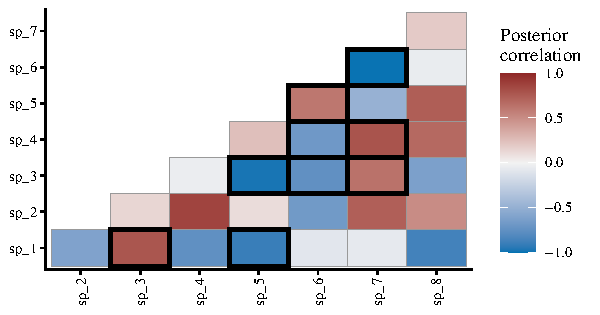
\includegraphics[width=\maxwidth]{figure/jsdgam-unnamed-chunk-4-1} 

}


\end{knitrout}

\texttt{\color{Orchid} ordinate(mod, rotation = 'varimax')}: a biplot of site scores and species loadings. A varimax rotation loads each species on as few factors as it can

\begin{knitrout}
\definecolor{shadecolor}{rgb}{0.969, 0.969, 0.969}\color{fgcolor}

{\centering 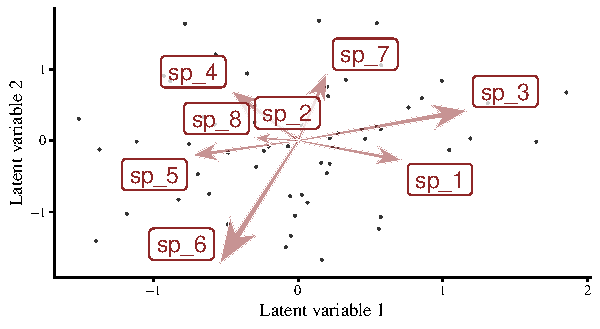
\includegraphics[width=\maxwidth]{figure/jsdgam-unnamed-chunk-5-1} 

}


\end{knitrout}

\texttt{\color{Orchid} shared\_variation(mod)}: the covariance the factors imply, with the variance each species shares on the diagonal. \texttt{\color{Orchid} compare\_loadings(mod1, mod2)} aligns the loadings of two fits

\smallskip
{{\fontsize{11}{11} \selectfont \color{mygray} How many factors?}}

\medskip
\texttt{\color{Orchid} active\_factors(mod)} gives the posterior probability that each factor is active under \texttt{\color{Orchid} loadings\_prior = 'mgp'}, here fitted with \texttt{\color{Orchid} n\_lv = 4}

\begin{knitrout}
\definecolor{shadecolor}{rgb}{0.969, 0.969, 0.969}\color{fgcolor}

{\centering 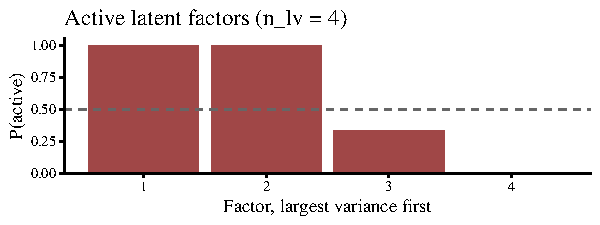
\includegraphics[width=\maxwidth]{figure/jsdgam-unnamed-chunk-6-1} 

}


\end{knitrout}

\end{block}
\end{column}


\begin{column}{.03\paperwidth}
\end{column}


\begin{column}{0.3\paperwidth}
\vspace{-0.15in}
\noindent\makebox[\linewidth]{\rule{0.3\paperwidth}{0.2pt}}
\begin{block}{{\fontsize{21}{21} \selectfont \color{BrickRed} Effects and prediction}}

\smallskip
{{\fontsize{11}{11} \selectfont \color{mygray} How does each species respond?}}

\medskip
\texttt{\color{Orchid} conditional\_effects(mod, effects = 'env:series')} plots the expected count of each species along \texttt{env}

\begin{knitrout}
\definecolor{shadecolor}{rgb}{0.969, 0.969, 0.969}\color{fgcolor}

{\centering 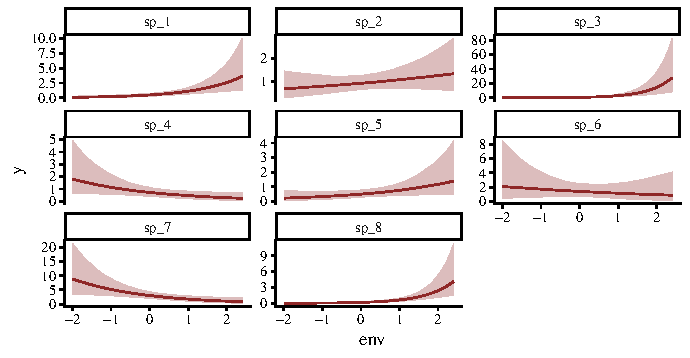
\includegraphics[width=\maxwidth]{figure/jsdgam-unnamed-chunk-7-1} 

}


\end{knitrout}

\smallskip
{{\fontsize{11}{11} \selectfont \color{mygray} Does the model predict well?}}

\medskip
\texttt{\color{Orchid} pp\_check(mod)}: simulated against observed responses, one panel per species with \texttt{\color{Orchid} type = 'dens\_overlay\_grouped'} and \texttt{\color{Orchid} group = 'series'}

\medskip
\texttt{\color{Orchid} kfold(mod, group = 'site')} holds out whole sites in turn and scores their expected log predictive density (higher is better). Each site's factor scores are estimated from a handful of observations. \texttt{\color{Orchid} loo(mod)} then often warns of high Pareto $k$

\medskip
A constrained ordination moves each factor with \texttt{env}. Each species then responds through its loadings. Compare it with free per-species slopes:
\begin{knitrout}
\definecolor{shadecolor}{rgb}{0.969, 0.969, 0.969}\color{fgcolor}\begin{kframe}
\begin{alltt}
\hldef{mod_con} \hlkwb{<-} \hlkwd{update}\hldef{(mod,} \hlkwc{formula.} \hldef{= y} \hlopt{~} \hldef{series,}
                  \hlkwc{factor_formula} \hldef{=} \hlopt{~ -}\hlnum{1} \hlopt{+} \hldef{env}\hlopt{:}\hlkwd{lv_axis}\hldef{())}
\end{alltt}
\end{kframe}
\end{knitrout}
\begin{knitrout}
\definecolor{shadecolor}{rgb}{0.969, 0.969, 0.969}\color{fgcolor}\begin{kframe}
\begin{alltt}
\hlkwd{print}\hldef{(}\hlkwd{loo_compare}\hldef{(mod, mod_con),} \hlkwc{p_worse} \hldef{=} \hlnum{FALSE}\hldef{)}
\end{alltt}
\begin{verbatim}
##    model elpd_diff se_diff
##      mod       0.0     0.0
##  mod_con     -18.1     4.9
\end{verbatim}
\end{kframe}
\end{knitrout}

\medskip
\texttt{\color{Orchid} posterior\_epred(mod, newdata = new\_sites)} predicts every species at unsurveyed sites from their covariates

\smallskip
{{\fontsize{11}{11} \selectfont \color{mygray} How do I report the model?}}

\medskip
\texttt{\color{Orchid} how\_to\_cite(mod)} drafts a methods paragraph with its references. \texttt{\color{Orchid} methods\_md(mod)} writes the model's equations and priors

\medskip
The \href{https://nicholasjclark.github.io/mvgam/dev/articles/jsdgam.html}{JSDM article} fits ant counts with traits, constrained ordination and factor shrinkage. The \href{https://github.com/nicholasjclark/mvgam/raw/master/misc/mvgam_cheatsheet.pdf}{mvgam cheatsheet} covers time-series models

\end{block}
\end{column}

\end{columns}
\end{frame}

\end{document}
